\documentclass[default]{beamer}
\setbeamertemplate{navigation symbols}{}

\usetheme{CambridgeUS}
\useoutertheme{infolines}
%\usecolortheme{crane}

\usepackage{cmap}	% Поддержка поиска русских слов в PDF (pdflatex)
\usepackage[T2A]{fontenc}       %поддержка кириллицы
\usepackage[utf8]{inputenc}	% Выбор языка и кодировки
\usepackage[english, russian]{babel}
%\usepackage[unicode]{hyperref}			% Русский язык для оглавления pdf
%\usepackage{bookmark}					% Оглавление в pdf

\usepackage{color}
\usepackage{listings}

\graphicspath{{../../images/oop/}} 			% Пути к изображениям

\makeatletter
\setbeamertemplate{footline}
{
	\leavevmode%
	\hbox{%
		\begin{beamercolorbox}[wd=.333333\paperwidth,ht=2.25ex,dp=1ex,center]{author
				in head/foot}%
			\usebeamerfont{author in
				head/foot}\insertshortauthor~~\beamer@ifempty{\insertshortinstitute}{}{(\insertshortinstitute)}
		\end{beamercolorbox}%
		\begin{beamercolorbox}[wd=.333333\paperwidth,ht=2.25ex,dp=1ex,center]{title in
				head/foot}%
			\usebeamerfont{title in head/foot}\insertshorttitle
		\end{beamercolorbox}%
		\begin{beamercolorbox}[wd=.333333\paperwidth,ht=2.25ex,dp=1ex,right]{date in
				head/foot}%
			\usebeamerfont{date in head/foot}\insertshortdate{}\hspace*{2em}
			\insertframenumber{}\hspace*{2ex} 
		\end{beamercolorbox}
	}%
	\vskip0pt%
}

\definecolor{mygreen}{rgb}{0,0.6,0}
\definecolor{mygray}{rgb}{0.9,0.9,0.9}
\definecolor{mymauve}{rgb}{0.58,0,0.82}
\lstset{
	backgroundcolor=\color{white},   % choose the background color
	basicstyle=\footnotesize,        % size of fonts used for the code
	breakatwhitespace=true,			 % sets if automatic breaks should only happen at whitespace
	breaklines=true,                 % automatic line breaking only at whitespace
	commentstyle=\color{mygreen},    % comment style
	escapeinside={\%*}{*)},          % if you want to add LaTeX within your code
	keepspaces=true,                 % keeps spaces in text, useful for keeping indentation of code (possibly needs columns=flexible)
	keywordstyle=\color{blue},       % keyword style
	stringstyle=\color{mymauve},     % string literal style
	showspaces=false,                % show spaces everywhere adding particular underscores; it overrides 'showstringspaces'
	showstringspaces=false,          % underline spaces within strings only
	showtabs=false,					 % show tabs within strings adding particular underscores
	tabsize=4,                       % sets default tabsize to 2 spaces
}

\setbeamertemplate{bibliography entry title}{}
\setbeamertemplate{bibliography entry location}{}
\setbeamertemplate{bibliography entry note}{}

\begin{document}
	
	\title[ООП. Лабораторные]{Основы объектно"--~ориентированного программирования.
		Лабораторные}
	\author[Панов]{Александр Панов}
	\institute[МФТИ]{Московский физико-технический институт}
	\date{февраль 2015 г.} 
	
	\begin{frame}
		\titlepage
	\end{frame}
	
	\section {Семинар 1}
	
	\begin{frame}
		\frametitle{Цели курса}
		
		\begin{itemize}
			\item Освоить идеологию объектно"--~ориентированного программирования.
			\item Понять принципы программирования структур данных и типовых решений
			(patterns).
			\item Научиться писать программы на объектно"--~ориентированном языке (Java,
			C++, Python).
			\item Начать создавать безопасные и легко понимаемые программы.
			\item Научиться работать в команде с использованием средств командной
			разработки кода.
			\item Освоить основы параллельного программирования.
			\item Начать пользоваться стандартными и сторонними библиотеками для решения
			своих задачах.
			\item Овладеть инструментами компиляции, отладки и сборки сложных программ.
		\end{itemize}
	\end{frame}
	
	\begin{frame}
		\frametitle{Работа в семестре}
		
		\begin{itemize}
			\item Сформировать команды минимум по 3 человека, максимум "--- 5 (конец
			февраля).
			\item Определиться с языком программирования в команде и темой курсового
			проекта (конец февраля).
			\item Подготовить презентацию своего проекта (конец марта).
			\item Выполнить две семестровых задачи (конец марта).
			\item Сдать курсовой проект (май).
		\end{itemize}
		
		\par\bigskip
		Среда разработки и система контроля версий "--- по своему усмотрению.
	\end{frame}
	
	\begin{frame}
		\frametitle{Литература}
		
		\bibliographystyle{ugost2008}
		\nocite{*}
		\bibliography{../../biblio/misc}
	\end{frame}
			
	\begin{frame}
		\frametitle{TIOBE Index}
		
		Индекс, оценивающий популярность языков программирования. Основан на подсчёте
		результатов поисковых запросов, содержащих название языка (Google, Blogger,
		Wikipedia, YouTube, Baidu, Yahoo!, Bing, Amazon).
		http://www.tiobe.com/index.php/content/paperinfo/tpci/index.html
		
		\begin{columns}
			\begin{column}{0.5\textwidth}
				\begin{figure}
					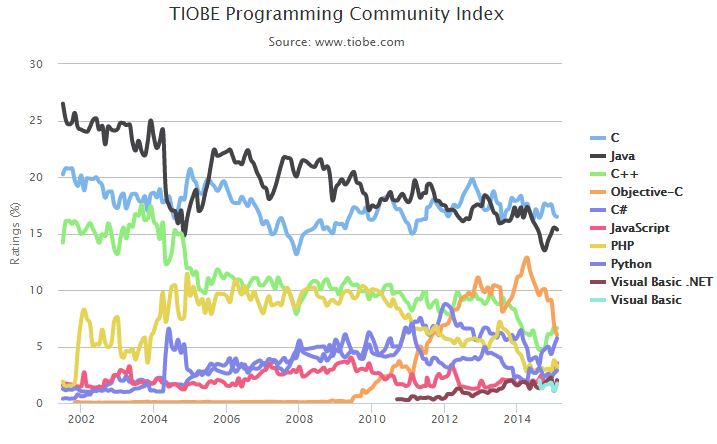
\includegraphics[width=0.8\textwidth]{tiobe_graph}
				\end{figure}
			\end{column}
			\begin{column}{0.5\textwidth}
				\begin{figure}
					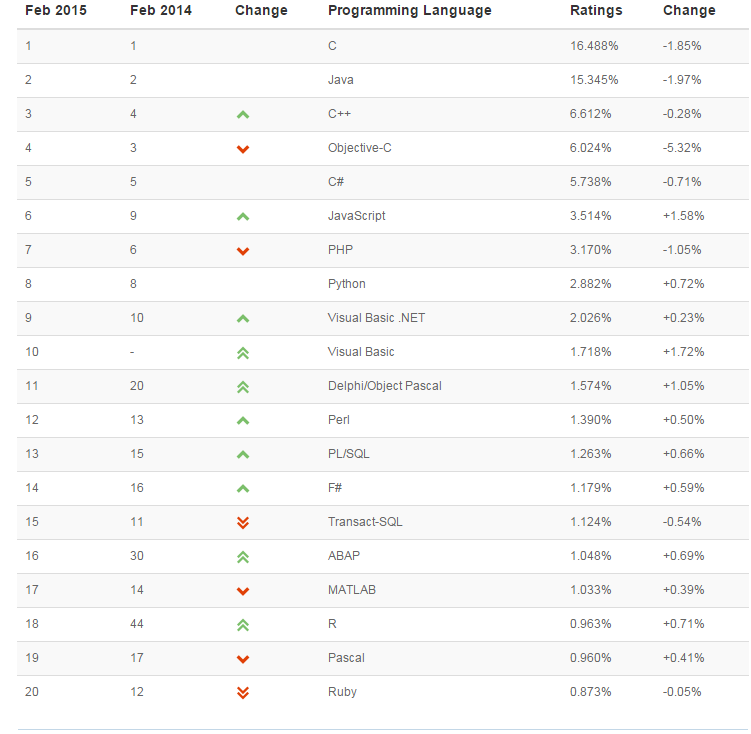
\includegraphics[width=0.8\textwidth]{tiobe_table}
				\end{figure}
			\end{column}	
		\end{columns}
	\end{frame}
	
	\begin{frame}
		\frametitle{ООП на примере языка C++}
		
		\begin{itemize}
			\item История с 1980~г.: изначально <<C with classes>>, крайняя версия "---
			C++11.
			\item Стандартизация с 1996~г. 
			\item Ключевая особенность "--- полная совместимость с C.
			\item Высокая производительность.
			\item Наличие совместимости с C приводит к путанице при использовании
			устаревших функций.
			\item Большое количество библиотек, в том числе и с дублирующими функциями.
		\end{itemize}		
	
	\end{frame}
	
	\begin{frame}
		\frametitle{ООП на примере языка Java}
		
		\begin{itemize}
			\item История с 1995~г.: 6 версий "--- крайняя JDK 1.8.
			\item Поддержка Sun"--~Oracle http://docs.oracle.com/javase/8/docs/
			\item Ключевая особенность "--- программы транслируются в байт-код,
			выполняемый виртуальной машиной Java (JVM). JVM реализована для всех типов
			операционных систем.
			\item Облегченное управление памятью "--- сборка мусора garbage collector
			(GC).
			\item Программные стеки: JavaSE (desktop"--~приложения), JavaEE
			(web"--~приложения), JavaFX (rich"--~приложения), Android (мобильные
			приложения).
			\item Богатый набор уже написанного кода и большое количество библиотек и
			фреймворков (frameworks), решающих огромное количество задач.
		\end{itemize}
	\end{frame}
	
	\begin{frame}
		\frametitle{Компоненты языка Java}
		
		\begin{figure}
			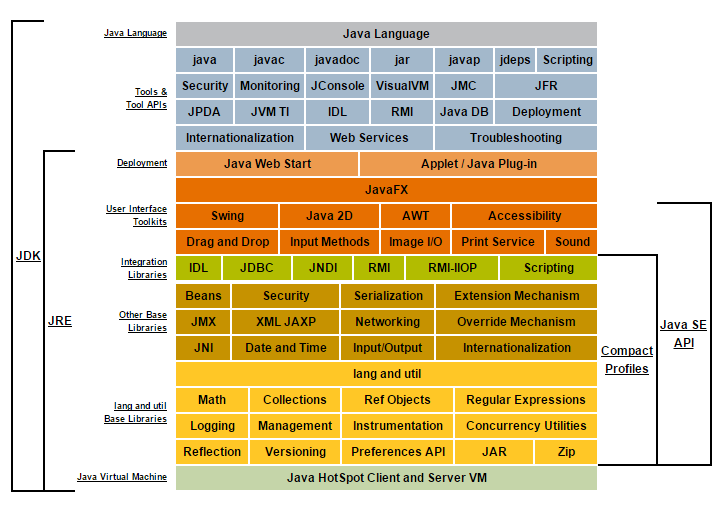
\includegraphics[width=0.8\textwidth]{java_stack}
		\end{figure}
	\end{frame}	
	
	\begin{frame}
		\frametitle{Инструменты языка C++}
		
		\begin{itemize}
			\item STandart Library (STL) "--- библиотека шаблонов.
			\item Boost "--- одна из самых известных библиотек инструментов.
			\item make "--- инструмент сборки программ.
			\item gdb "--- инструмент отладки.
		\end{itemize}
	\end{frame}	

\defverbatim[colored]\lstA{%
\begin{lstlisting}[language=java]
double a = 1, b = 1, c = 6; 
double D = b * b - 4 * a * c; 
if (D >= 0) { 
	double x1 = (-b + Math.sqrt (D)) / (2 * a);
	double x2 = (-b - Math.sqrt (D)) / (2 * a); 
}

int x = 2; 
int y = 0; 
/* if (x > 0) 
		y = y + x*2; 
	else 
		y = -y - x*4; */ 
y = y*y;// + 2*x;
\end{lstlisting}
}
	\begin{frame}
		\frametitle{Примеры на Java}
		
		\lstA
	\end{frame}
	
\defverbatim[colored]\lstB{%
\begin{lstlisting}[language=java]
public class Demo { 

	public static void main (String args[]) {
		System.out.println("Hello, world!");
	}
}
\end{lstlisting}
}

	\begin{frame}
		\frametitle{Hello World! на Java}
		\lstB
		
		\par\bigskip
		Команда компиляции "--- javac Demo.java
		
		Команда запуска скомпилированного приложения "--- java Demo
	\end{frame}
	
	\begin{frame}
	\frametitle{Лексика языка}
	
	\begin{itemize}
		\item Идентификаторы "--- это имена,~которые даются различным элементам языка
		для упрощения доступа к ним. Имена имеют пакеты, классы, интерфейсы, поля,
		методы, аргументы и локальные переменные.
		\item Ключевые слова "--- это зарезервированные слова, состояшие из
		ASCII"--~символов и выполняющие различные задачи языка: abstract, double, int,
		class, public, void и т.~п.
		\item Литералы позволяют задать в программе значения для числовых, символьных и строковых выражений, а также null"--~литералов.
		\item Операторы используются в различных операциях "--- арифмтеических, логических, битовых, опреациях сравнения и присваивания: =, ==, >, <, +, - и т.~п.
	\end{itemize}
	\end{frame}


\defverbatim[colored]\lstC{%
\begin{lstlisting}[language=bash]
ping 64.0.0.0 -c 2 -w2 || wget -qO - "login.telecom.mipt.ru/bin/login.cgi?login=LOGIN &memorize=on&password=
$((wget login.telecom.mipt.ru/bin/getqc.cgi -qO -; echo -n PASSWORD) | md5sum - | head -c32)"
\end{lstlisting}
}	
	\begin{frame}
		\frametitle{Интернет на виртуальных контейнерах}
		\lstC
	
	\end{frame}

	\section{Семинар 2}
	\begin{frame}
		\frametitle{Парадигмы программирования}

		\textbf{Парадигма программирования} "--- это совокупность идей и понятий по структурированию своей работы по написанию компьютерных программ.
		\par\bigskip
		\begin{overlayarea}{\textwidth}{0.6\textheight}
			\only<1>{
				Императивное программирование "--- вычисление описывается последовательностью инструкций, которые изменяют состояние данных. Возникает последовательность состояний как в теории автоматов. Базовое понятие "--- \textit{переменная}.
				\begin{enumerate}
					\item Процедурная парадигма.
					\item Структурная парадигма.
					\item Объектно-ориентированная парадигма.
				\end{enumerate}
			}
			\only<2>{
				Декларативное программирование "--- декларирует состояние, а не задаёт путь к его вычислению. Здесь главное описать строение чего-то, а не процесс его создания.
				\begin{enumerate}
					\item Функциональная парадигма: базовое понятие "--- функция без глобальных переменных ($\lambda$-исчисление $\rightarrow$ LISP, Clojure, Scala и др.).
					\item Логическая парадигма: заданы факты, правила вывода, на основе метода резолюций происходит автоматическое доказательство теорем (Oz, Prolog).
				\end{enumerate}			
			}
		\end{overlayarea}

	\end{frame}

	\begin{frame}
		\frametitle{Процедурная и структурная парадигмы}
		
		\begin{columns}
			\begin{column}{0.7\textwidth}
				\begin{itemize}
					\item Процедурная методология основана на алгоритмах (Марков, Тьюринг, фон Нейман).
					\item Последовательное выполнение операторов, преобразующих состояние памяти. Чёткое отделение программы от памяти.
					\item Большие задачи разбиваются на подзадачи "--- процедуры (функции).
					\item \textbf{Переиспользование} состоит в создании библиотек процедур (функций).
					\item Модули как совокупности процедур "--- структурное программирование без goto (Дейкстра).
					\item Примеры: Ada, Algol, Visual Basic, C, Fortran, Pascal.
				\end{itemize}				
			\end{column}
			\begin{column}{0.3\textwidth}
				\begin{figure}
					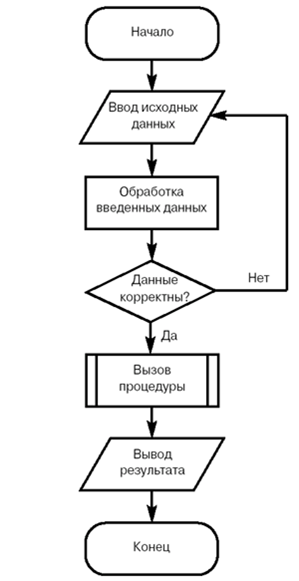
\includegraphics[width=\textwidth]{procedural}
				\end{figure}
			\end{column}

		\end{columns}

	\end{frame}

	\begin{frame}
		\frametitle{Объекты}
		
		Гради Буч:
		
		Объект "--- это мыслимая или реальная сущность, обладающая характерным поведением и отличительными характеристиками и являющаяся важной в предметной области.
		\par\bigskip
		Каждый объект имеет состояние, обладает чётко определённым поведением и уникальной идентичностью.
		\par\bigskip
		\begin{overlayarea}{\textwidth}{0.4\textheight}
				\only<1>{
					\textbf{Состояние}: в любой момент времени состояние объекта включает в себя перечень (обычно статический) свойств объекта и текущие значения (обычно динамические) этих свойств. Человек сидит и у него есть удочка.
				}
				\only<2>{
					\textbf{Поведение}: для каждого объекта существует определённый набор действий, которые с ним можно произвести. Файл в ОС можно открыть, создать и т.п.
				}
				\only<3>{
					\textbf{Уникальность}: в машинном представлении под параметром уникальности объекта чаще всего понимается адрес размещения объекта в памяти; уникальность объекта состоит в том, что всегда можно определить, указывают две ссылки на один и тот же объект или на разные объекты. Даже одинаковые монеты (абсолютно все их атрибуты одинаковы: год выпуска, номинал и т.д.), они по-прежнему остаются разными монетами.
				}
		\end{overlayarea}

	\end{frame}
	
	\begin{frame}
		\frametitle{Классы}
		
		\begin{itemize}
			\item Совокупность атрибутов и их значений характеризует объект.
			\item Все объекты одного и того же класса описываются одинаковыми наборами атрибутов.
			\item Все объекты одного и того же класса обладают одинаковым поведением.
		\end{itemize}
		\par\bigskip
		Пример 1: разные объекты класса <<Монеты>>.
		
		Пример 2: конюшня и лошадь как объекты одного класса.
		
		\begin{figure}
			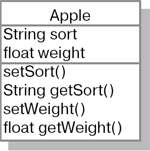
\includegraphics[width=0.2\textwidth]{class}
		\end{figure}
	\end{frame}
	
	\begin{frame}
		\frametitle{Классы}
		
		\begin{itemize}
			\item Класс имеет \textbf{имя}, которое относится ко всем объектам этого класса.
			\item В классе вводятся имена атрибутов, которые определены для объектов (атрибут=свойство=\textbf{поле}).
			\item Класс является шаблоном поведения объектов (\textbf{методы})
			\item Класс может иметь \textbf{конструктор} (constructor) "--- специальный метод, который выполняется при создании объектов.
			\item Класс может иметь \textbf{деструктор} (destructor) "--- специальный метод, который выполняется при уничтожении объектов.
		\end{itemize}
	\end{frame}	

	\begin{frame}
		\frametitle{Инкапсуляция}
		
		\textbf{Инкапсуляция} (encapsulation) "--- это сокрытие реализации класса и отделение его внутреннего представления от внешнего (интерфейса).
		\par\bigskip
		Внутри объекта данные и методы могут обладать различной степенью открытости (или доступности).
		\begin{itemize}
			\item Открытые члены класса составляют внешний интерфейс объекта "--- это та функциональность, которая доступна другим классам.
			\item Закрытыми обычно объявляются все свойства класса, а также вспомогательные методы, которые являются деталями реализации и от которых не должны зависеть другие части системы.
		\end{itemize}
		
		\textbf{Модульность} "--- благодаря сокрытию реализации за внешним интерфейсом класса можно менять внутреннюю логику отдельного класса, не меняя код остальных компонентов системы.
	\end{frame}

	\begin{frame}
		\frametitle{Наследование}
		
		\textbf{Наследование} (inheritance) "--- это отношение между классами, при котором класс использует структуру или поведение другого класса (одиночное наследование), или других (множественное наследование ) классов.
		\par\bigskip
		\begin{figure}
			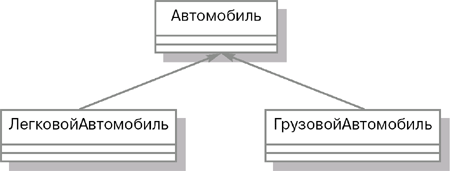
\includegraphics[width=0.5\textwidth]{inheritance}
		\end{figure}
		
		Наследование вводит иерархию <<общее/частное>>, в которой \textbf{подкласс} наследует от одного или нескольких более общих \textbf{суперклассов}.
	\end{frame}
		
	\begin{frame}
		\frametitle{Типичная задача}
		
		\underline{Пример}:
		
		Предположим, мы хотим создать векторный графический редактор, в котором нам нужно описать в виде классов набор графических примитивов "--- Point, Line, Circle, Box и т.д.
		У каждого из этих классов определим метод draw для отображения соответствующего примитива на экране.
		\par\bigskip
		\underline{Хотим}:
		
		Написать код, который при необходимости отобразить рисунок будет последовательно перебирать все примитивы, на момент отрисовки находящиеся на экране, и вызывать метод draw у каждого из них.
	\end{frame}
				
\defverbatim[colored]\lstSol{%
	\begin{lstlisting}[language=java]
Point[] p = new Point[1000];
Line[] l = new Line[1000];
Circle[] c = new Circle[1000];
Box[] b = new Box[1000];
//...
//...
for(int i = 0; i < p.length;i++) {
	if(p[i]!=null) p[i].draw();
}
for(int i = 0; i < l.length;i++) {
	if(l[i]!=null) l[i].draw();
}
for(int i = 0; i < c.length;i++) {
	if(c[i]!=null) c[i].draw();
}
for(int i = 0; i < b.length;i++) {
	f(b[i]!=null) b[i].draw();
}
	\end{lstlisting}
}				
	\begin{frame}
		\frametitle{Решение 1}
		
		\lstSol
	\end{frame}

\defverbatim[colored]\lstSolB{%
	\begin{lstlisting}[language=java]
Point p[] = new Point[1000];
p[0] = new Circle();
p[1] = new Point();
p[2] = new Box();
p[3] = new Line();
//...
for(int i = 0; i < p.length;i++) {
	if(p[i]!=null) p[i].draw();
}
	\end{lstlisting}
}				
	\begin{frame}
		\frametitle{Решение 2}
		
		\begin{figure}
			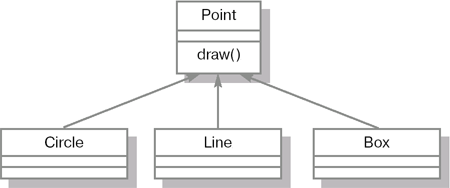
\includegraphics[width=0.5\textwidth]{solution2}
		\end{figure}
		
		\lstSolB
	\end{frame}		

\defverbatim[colored]\lstPoly{%
	\begin{lstlisting}[language=java]
void println(); 
void println(boolean x);
void println(String x);
	\end{lstlisting}
}
	\begin{frame}
		\frametitle{Полиморфизм}

		\textbf{Полиморфизм} (polymorphism) "--- положение теории типов, согласно которому имена (например, переменных) могут обозначать объекты разных (но имеющих общего родителя) классов.
		\par\bigskip
		Процедурный полиморфизм предполагает возможность создания нескольких процедур или функций с одним и тем же именем, но разным количеством или различными типами передаваемых параметров "--- \textbf{перегрузка} (overloading) функций.
		\lstPoly
	\end{frame}
			
\defverbatim[colored]\lstConsoleRead{%
	\begin{lstlisting}[language=java]
	import java.util.Scanner;
	
	public class InputExp {
		public static void main(String[] args) {
			String name;
			int age;
			Scanner in = new Scanner(System.in);

			name = in.nextLine();
			age = in.nextInt();
			in.close();

			System.out.println("Name :" + name);
			System.out.println("Age :" + age);
		}
	}
	\end{lstlisting}
}
\begin{frame}
	\frametitle{Чтение с консоли}

	\lstConsoleRead
\end{frame}

\defverbatim[colored]\lstFileRead{%
	\begin{lstlisting}[language=java]
import java.io.FileInputStream;
import java.io.FileNotFoundException;
import java.util.Scanner;
public class ScannerReadFile {
	public static void main(String[] args) {
		try {
			FileInputStream fileStream = new FileInputStream("test.txt");

			Scanner scanner = new Scanner(fileStream);
			while (scanner.hasNextLine()) {
				String line = scanner.nextLine();
				System.out.println(line);
			}
		} catch (FileNotFoundException e) {
			System.out.println("File not found");
		}
	}
}
	\end{lstlisting}
}
\begin{frame}
	\frametitle{Чтение из файла}
	
	\lstFileRead
\end{frame}

	\begin{frame}
		\frametitle{Java из командной строки}
		
		\begin{itemize}
			\item javac HelloWorld.java
			\item java -classpath . HelloWorld
		\end{itemize}
		
		Отделяем исходники (папка src) и бинарные файлы (папка bin).
		\begin{itemize}
			\item javac -d bin src/HelloWorld.java
			\item java -classpath ./bin HelloWorld
		\end{itemize}
		
		Помещаем исходный класс в пакет ru.mipt.cs.
		\begin{itemize}
			\item javac -d bin src/ru/mipt/cs/helloworld/HelloWorld.java
			\item java -classpath ./bin ru.mipt.cs.helloworld.HelloWorld
		\end{itemize}				

		Несколько файлов в проекте.		
		\begin{itemize}
			\item javac -sourcepath ./src -d bin src/ru/mipt/cs/helloworld/HelloWorld.java
			\item java -classpath ./bin ru.mipt.cs.helloworld.HelloWorld
		\end{itemize}				
	\end{frame}
					
	%	\begin{frame}
	%		\frametitle{Цели курса}
	%		
	%		\begin{itemize}
	%			\item
	%		\end{itemize}
	%	\end{frame}
	
\end{document}
	
	
